\documentclass{article}%
\usepackage[T1]{fontenc}%
\usepackage[utf8]{inputenc}%
\usepackage{lmodern}%
\usepackage{textcomp}%
\usepackage{lastpage}%
\usepackage{authblk}%
\usepackage{graphicx}%
%
\title{Expression and Differentiation between OCT4A and Its Pseudogenes in Human ESCs and Differentiated Adult Somatic Cells}%
\author{Erica Douglas}%
\affil{Advanced Laboratory for Plant Genetic Engineering, Advanced Technology Development Centre, Indian Institute of Technology Kharagpur, Kharagpur, India}%
\date{01{-}01{-}2009}%
%
\begin{document}%
\normalsize%
\maketitle%
\section{Abstract}%
\label{sec:Abstract}%
The biological trigger that is essential for Ellipticine to progress to lung cancer is a favorable Akt translocation, or conversion from normal to lethal in lung epithelial cancer cells, researchers say. Ellipticine stimulates Akt translocation and signals the activation of signaling proteins produced by the progenitor of cancer cell xenografts.\newline%
Proteins that are more abundant in xenografts than normal cells give the researchers a valuable window into the progression of the disease.\newline%
In an Amherst College study published in Nature Cell Biology, researchers reported how Ellipticine induces Akt translocation by activating genes that encodes the docking protein YM, a transcription factor that maintains the protective membrane of VEGF, a regulatory protein involved in placental growth. Among other things, YM is found in the genetic messengers and related proteins that regulate cell behavior, such as the hid in the egg cell.\newline%
When cells produced by mice are infected with Ellipticine, abnormal T{-}cells that express YM modify their normal cytotoxic activities, translating them into an endotoxin and subsequently tumor cells. When T{-}cells are treated with Ellipticine and subjected to the FGF vaccine in normal cells, abnormal T{-}cells do not have the response necessary to reconstitute T{-}cells.\newline%
Using this information, the researchers calculated that 30 percent of the attacks on T{-}cells was because of Akt translocation.\newline%
The results from their study were reported in the December 2010 issue of the journal Cell Biology.\newline%
The researchers and their collaborators were a group of researchers from the Woods Hole Medical Research Institute in Woods Hole, Mass., Harvard Medical School in Cambridge, Mass., and Fred Hutchinson Cancer Research Center in Seattle, Wash.

%
\subsection{Image Analysis}%
\label{subsec:ImageAnalysis}%


\begin{figure}[h!]%
\centering%
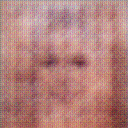
\includegraphics[width=150px]{500_fake_images/samples_5_223.png}%
\caption{A Close Up Of A Person Holding A Pair Of Scissors}%
\end{figure}

%
\end{document}